\documentclass[12pt]{article}
\usepackage{csquotes}
\usepackage{blindtext}
\usepackage{titling}
\usepackage[papersize={8.5in,11in}, margin=1in]{geometry}
\usepackage{amsmath}
\usepackage{amssymb}
\usepackage{graphicx}
\usepackage{float}
\usepackage{subcaption}
\usepackage{booktabs}
\usepackage{parskip}
\usepackage{adjustbox}
\usepackage{hyperref}
\usepackage{amsfonts}
\usepackage{float}
\usepackage{sourcecodepro}
\usepackage[T1]{fontenc}
\usepackage{listings}
\usepackage{mathpartir}
\usepackage[english]{babel}

\usepackage{graphicx, amsmath, amsfonts, amssymb, enumerate, amsthm, commath, float, xcolor}
% Useful packages
\usepackage{amsmath}
\usepackage{amssymb}
\usepackage{graphicx}
\usepackage{listings}
\usepackage{xcolor}
\usepackage{float}
% \usepackage[colorlinks=true, allcolors=blue]{hyperref}

\lstset{basicstyle=\ttfamily}
\hypersetup{
    colorlinks=true,
    linkcolor=blue,
    filecolor=magenta,      
    urlcolor=cyan,
    citecolor=black,
    pdfpagemode=FullScreen,
}
\usepackage[backend=biber, style=alphabetic, sorting=ynt]{biblatex}
\addbibresource{bib.bib}

\usepackage{algpseudocode}
\usepackage{algorithm}


\begin{document}

\begin{titlepage}

  \newcommand{\HRule}{\rule{\linewidth}{0.5mm}}

  \center

  
\includegraphics[width=250px, keepaspectratio]{./columbia-logo.png}\\[1cm]
  \textsc{\Large Research Project}\\[0.5cm]
  \textsc{\large COMS 4901}\\[0.3cm]
  \textsc{\large Prof. Stephen Edwards and John Hui}\\[0.5cm]

  \HRule \\[0.4cm]
  { \huge \bfseries Implementation of two solutions to the Order Maintenance Problem}\\[0.4cm]
  \HRule \\[1.5cm]

  \begin{minipage}{0.4\textwidth}
    \begin{center} \large
      Alexis \textsc{Gadonneix} (ag4625)\\
    \end{center}

  \end{minipage}\\[2cm]

  {\large December 2023}\\[2cm]

  \vfill

\end{titlepage}

\section{Tests}

Blabla

\begin{lstlisting}
	fn test() {
		code = working;
	}
\end{lstlisting}

maths:
\begin{equation}
  \begin{aligned}
    \text{minimize} \quad   & \sum_{i=1}^{n} \sum_{j=1}^{n} c_{ij} x_{ij}       \\
    \text{subject to} \quad & \sum_{i=1}^{n} x_{ij} = 1, \quad j = 1, \dots, n, \\
                            & \sum_{j=1}^{n} x_{ij} = 1, \quad i = 1, \dots, n, \\
                            & x_{ij} \in \{0, 1\}, \quad i,j = 1, \dots, n.
  \end{aligned}
\end{equation}

\newpage
\section{Introduction}

The order maintenance problem is a well-known problem in computer science. It is defined as follows: given a set of elements, we want to maintain a data structure that supports the following operations:
\begin{itemize}
  \item \texttt{insert(x)}: insert a new element right after \texttt{x}
  \item \texttt{delete(x)}: delete \texttt{x}
  \item \texttt{compare(x, y)}: which element of \texttt{x} and \texttt{y} has higher priority?
\end{itemize}

A first very crude solution to this problem is to use a vector. But all operations are linear in the size of the vector. We can do better.
A better idea would be to use a linked list. But then, the \texttt{compare} operation is linear in the size of the list...

This data structure has several applications in computer science such as process scheduling and graph algorithms.
We will focus on two data structures to solve this problem: The firstwas proposed by Dietz \& Sleator in 1987 \cite{10.1145/28395.28434} and the second by Bender et al. in 2002 \cite{10.5555/647912.740822}.
The two solutions have very similar theoretical bounds, but the second one is more practical.

The main goals of this project are:
\begin{itemize}
  \item Implement both solutions in Rust
  \item Test and debug
  \item Benchmark, compare, and optimize
\end{itemize}

\newpage
\section{Algorithms}

\subsection{Naive}

Before diving into the two solutions, let's look at a naive solution to the problem.
We can store our priorities in a binary tree that grows deeper and deeper as we insert elements.
To avoid having to maintain an actual tree, we can simply use the labels of the nodes:
\begin{itemize}
  \item The first priority is labeled 0
  \item When we do an \texttt{insert(x)}, we relabel \texttt{x} to be $2 \times \texttt{label(x)}$ and the new element has label $2 \times \texttt{label(x)} + 1$
  \item The comparison between two elements is simply a comparison of their labels
\end{itemize}

TODO: insert image

This solution is easy to implement and operations are fast, but it has a major drawback: the labels grow exponentially with the number of insertions and will quickly overflow.

\subsection{Dietz \& Sleator}

In the solution proposed by Dietz \& Sleator in 1987 \cite{10.1145/28395.28434}, we think of the set of possible labels (e.g. $0$ to $2^{64}$) as a circular list that we will fill in as we insert elements.
The priorities are connected together by a circular doubly-linked list.
The general idea for inserting a new priority after a priority \texttt{x} is the following (see algorithm TODO for more details):
\begin{itemize}
  \item We iterate through the successors of \texttt{x} and compute a weight for each of them based on the distance between the elements
  \item We stop when we reach an element whose weight is smaller than a threshold (intuitively, this means that the element is "far enough")
  \item We then relabel those elements evenly
  \item Finally, we choose a label in between the labels of \texttt{x} its successor (in the middle) and we create a new priority with this label
\end{itemize}

We call this algorithm \textbf{list-range relabeling}.

TODO: insert image

Note that to avoid overflowing, we will simply loop back to 0 when we reach the maximum label ($2^{64}$).
But this means that in order to compare two elements, we have to keep track of a "base" label starting at 0 and shifting if necessary.
Then, the comparison operation is:
$$ (\texttt{label(x)} - \texttt{label(base)}) \quad \text{mod} \quad 2^{64} < (\texttt{label(y)} - \texttt{label(base)}) \quad \text{mod} \quad 2^{64} $$

Deleting an element of the data structure is as simple as removing it from the linked list.

The paper proves the following theoretical complexity bounds (where $n$ is the number of elements in the data structure):
\begin{itemize}
  \item \texttt{insert(x)}: $O(\log n)$ (amortized)
  \item \texttt{delete(x)}: $O(1)$
  \item \texttt{compare(x, y)}: $O(1)$
\end{itemize}

It is possible to get an $O(1)$ amortized complexity for \texttt{insert(x)} by adding a level of indirection using a technique by Tsakalidis \cite{10.1007/BFb0036494}. We chose not to implement this extra-layer for the sake of simplicity and because we thought that the complexity gains would be too small in comparison to the cost of the extra lookup.

This data structure theoretically only supports $\sqrt{M}$ insertions where $M$ is the number of possible labels ($2^32$ or $2^{64}$). It is a significant limitation on a $32$-bits machine as you can insert at most $65$K priorities.

\subsection{Bender et al.}

In 2002, Bender et al. proposed a new solution to the problem in \cite{10.5555/647912.740822}. The main goal of this approach is not to provide better bounds, but to get an algorithm and a proof that are more intuitive. In practice, we will see that our implementation is in fact faster than the first algorithm for some operations.

This time, we look at the set of possible labels ($0$ to $2^{64}$) as the leaves of a binary tree whose root is the empty string, and each node $n$ has two children $n:0 = 2 \times n$ and $n:1 = 2 \times n + 1$ (where $:$ is the concatenation to the binary representation).
We don't have to maintain an explicit tree because we can easily compute the parent or the children of a node with bit operations.
And once again, the priorities (which are leaves of the implicit tree) are connected together by a doubly-linked list (this one doesn't need to be circular).

The algorithm for \texttt{insert(x)} is pretty straightforward (ref algo TODO), and the key steps are:

\begin{itemize}
  \item if there is space ($\texttt{label(next(x))} > \texttt{label(x)} + 1$), then just insert the new element somewhere in between.
  \item if there is no space available, we have to relabel (we call this algorithm \textbf{tag-range relabeling}).
        \begin{itemize}
          \item To do so, we simply have to go up the tree and find the first sub-tree containing \texttt{x} that is not "too dense".
          \item Once we find this sub-tree, we simply have to spread evenly all the elements it contains over the range of labels the sub-tree. Note that once again, all these operations can be done with simple bit operations over the labels.
        \end{itemize}
\end{itemize}

TODO: Insert image

The paper proves that this algorithm has the same complexity bounds as the previous one:
\begin{itemize}
  \item \texttt{insert(x)}: $O(\log n)$
  \item \texttt{delete(x)}: $O(1)$
  \item \texttt{compare(x, y)}: $O(1)$
\end{itemize}

The same indirection trick can be applied to reduce the insertion complexity, but we chose not to implement it for the same reasons as before.

Deleting an element of the data structure is as simple as removing it from the linked list.
And a small but important difference is that, in order to compare two elements, we simply have to compare their labels (and we don't have to compute their position relative to a base as in the previous solution).

The previous data structure was limited to $\sqrt{M}$ insertions. Here, the maximum number of elements you can insert depends on the parameter $T$. If $T$ is close to $2$, the insertion will be faster but you can only insert a small amount of priorities before the root overflows. If $T$ is close to $1$, the algorithm is slower but you can insert more priorities (close to $M$).
The issue is that it's difficult to find a good trade-off as the user doesn't usually know up-front how many priorities he will need.
But the good news is that $T$ doesn't have to be fixed and you can compute the best $T$ at each insertion.
This computation is not free though, and we will see later (TODO ref to relevant section) how we made this process faster.

\newpage
\section{Implementation}

In this section, I will present the main data structures and design choices of our implementations, as well as some tricks we used to improve the speed.

\subsection{Interface}

The project was built as a Rust library (a \lstinline{cargo crate}). In order to have a common interface for multiple implementations, as well as shared tests and benchmarks, we leveraged Rust's \lstinline{Trait} system. The interface for a priority is minimal:
\begin{itemize}
  \item \lstinline{new: () -> Priority}: create a new priority, unrelated to any other priority
  \item \lstinline{insert: Priority -> Priority}: insert a new priority right after the argument
\end{itemize}

The comparison is made possible through the implementation of the \lstinline{PartialCmp} trait which lets us use the common comparison operators (\lstinline{>=}, \lstinline{<}, etc.).

The deletion is implemented through the \lstinline{Drop} trait, which acts as a destructor. A priority is deleted from the data structure when it goes out of scope.

\subsection{Common data structures}

I won't go too much into the technical details, but we used a couple of data structures to implement both solutions (\cite{10.5555/647912.740822} and \cite{10.1145/28395.28434}).

\begin{itemize}
  \item \lstinline{PriorityInner} is a node of a circular doubly-linked list. It can be seen as the private interface of a \lstinline{Priority}. It stores the following fields: \lstinline{prev}, \lstinline{next}, \lstinline{label}, \lstinline{ref_count}. The first two are (smart) pointers to the neighbors, the third is the label as a \lstinline{usize = u64} (on a 64-bit machine), and the last one is used for the manual reference counting. Those fields are actually wrapped in smart pointers called \lstinline{RefCell}, mutable memory locations. It is necessary to abide by Rust's borrow checker when trying to mutate a field of an object that is not owned or borrowed as mutable (this is called the interior mutability pattern).
  \item \lstinline{Arena} is the internal store of priorities containing all the \lstinline{PriorityInner}. In our case, it's a \lstinline{Slab}. It is indexed by \lstinline{PriorityKey}, an alias for \lstinline{usize}. The implementation of the \lstinline{Arena} contains all the methods in charge of creating, deleting, and connecting the \lstinline{PriorityInner}, the nodes of the linked list.
\end{itemize}

The end-user has access to a \lstinline{Priority}, which contains (privately) its \lstinline{PriorityKey} and a reference to the \lstinline{Arena}.

\subsection{Pre-compute the density thresholds}

\newpage
\section{Testing, Benchmarking, and results}

\subsection{Unit tests, Integration tests, and Quickcheck}

\subsection{Bugs found and fixed}

Overflow issue DnS

min and max labels overflow Bender

\subsection{Benchmarks, Profiling, and Optimization}


\newpage
\section{Conclusion and Future Work}

\begin{itemize}
  \item Test and benchmark on a microcontroller
  \item Try different allocation strategies
  \item Implement a "naive start" for small use cases
\end{itemize}

\newpage
\printbibliography

\end{document}

\documentclass[12pt]{article}
\usepackage{csquotes}
\usepackage{blindtext}
\usepackage{titling}
\usepackage[papersize={8.5in,11in}, margin=1in]{geometry}
\usepackage{amsmath}
\usepackage{amssymb}
\usepackage{graphicx}
\usepackage{float}
\usepackage{subcaption}
\usepackage{booktabs}
\usepackage{parskip}
\usepackage{adjustbox}
\usepackage{hyperref}
\usepackage{amsfonts}
\usepackage{float}
\usepackage{sourcecodepro}
\usepackage[T1]{fontenc}
\usepackage{listings}
\usepackage{mathpartir}
\usepackage[english]{babel}

\usepackage{graphicx, amsmath, amsfonts, amssymb, enumerate, amsthm, commath, float, xcolor}
% Useful packages
\usepackage{amsmath}
\usepackage{amssymb}
\usepackage{graphicx}
\usepackage{listings}
\usepackage{xcolor}
\usepackage{float}
% \usepackage[colorlinks=true, allcolors=blue]{hyperref}

\lstset{basicstyle=\ttfamily}
\hypersetup{
  colorlinks=true,
  linkcolor=blue,
  filecolor=magenta,
  urlcolor=cyan,
  citecolor=black,
  pdfpagemode=FullScreen,
}
\usepackage[backend=biber, style=alphabetic, sorting=ynt]{biblatex}
\addbibresource{bib.bib}

\usepackage{algpseudocode}
\usepackage{algorithm}
\algrenewcommand{\algorithmiccomment}[1]{\hfill// #1}


\begin{document}

\begin{titlepage}

  \newcommand{\HRule}{\rule{\linewidth}{0.5mm}}

  \center

  
\includegraphics[width=250px, keepaspectratio]{./columbia-logo.png}\\[1cm]
  \textsc{\Large Research Project}\\[0.5cm]
  \textsc{\large COMS 4901}\\[0.3cm]
  \textsc{\large Prof. Stephen Edwards and John Hui}\\[0.5cm]

  \HRule \\[0.4cm]
  { \huge \bfseries Implementation of two solutions to the Order Maintenance Problem}\\[0.4cm]
  \HRule \\[1.5cm]

  \begin{minipage}{0.4\textwidth}
    \begin{center} \large
      Alexis \textsc{Gadonneix} (ag4625)\\
    \end{center}

  \end{minipage}\\[2cm]

  {\large December 2023}\\[2cm]

  \vfill

\end{titlepage}


\section{Introduction}

The order maintenance problem is a well-known problem in computer science. It is defined as follows: given a set of elements, we want to maintain a data structure that supports the following operations:
\begin{itemize}
  \item \texttt{insert(x)}: insert a new element right after \texttt{x}
  \item \texttt{delete(x)}: delete \texttt{x}
  \item \texttt{compare(x, y)}: which element of \texttt{x} and \texttt{y} has higher priority?
\end{itemize}

A first very crude solution to this problem is to use a vector. But all operations are linear in the size of the vector. We can do better.
A better idea would be to use a linked list. But then, the \texttt{compare} operation is linear in the size of the list...

This data structure has several applications in computer science such as process scheduling and graph algorithms.
We will focus on two data structures to solve this problem: The first was proposed by Dietz \& Sleator in 1987 \cite{10.1145/28395.28434} and the second by Bender et al. in 2002 \cite{10.5555/647912.740822}.
The two solutions have very similar theoretical bounds, but the second one is more practical.

The main goals of this project are:
\begin{itemize}
  \item Implement both solutions in Rust
  \item Test and debug
  \item Benchmark, compare, and optimize
\end{itemize}

\newpage
\section{Algorithms}

\subsection{Naive}

Before diving into the two solutions, let's look at a naive solution to the problem.
We can store our priorities in a binary tree that grows deeper and deeper as we insert elements (see Figure \ref{naive} for an example).
To avoid having to maintain an actual tree, we can simply use the labels of the nodes:
\begin{itemize}
  \item The first priority is labeled 0
  \item When we do an \texttt{insert(x)}, we relabel \texttt{x} to be $2 \times \texttt{label(x)}$ and the new element has label $2 \times \texttt{label(x)} + 1$
  \item The comparison between two elements is done by finding the ancestor of the deepest element that is at the same depth as the other one, and comparing these.
\end{itemize}


\begin{figure}[h!]
  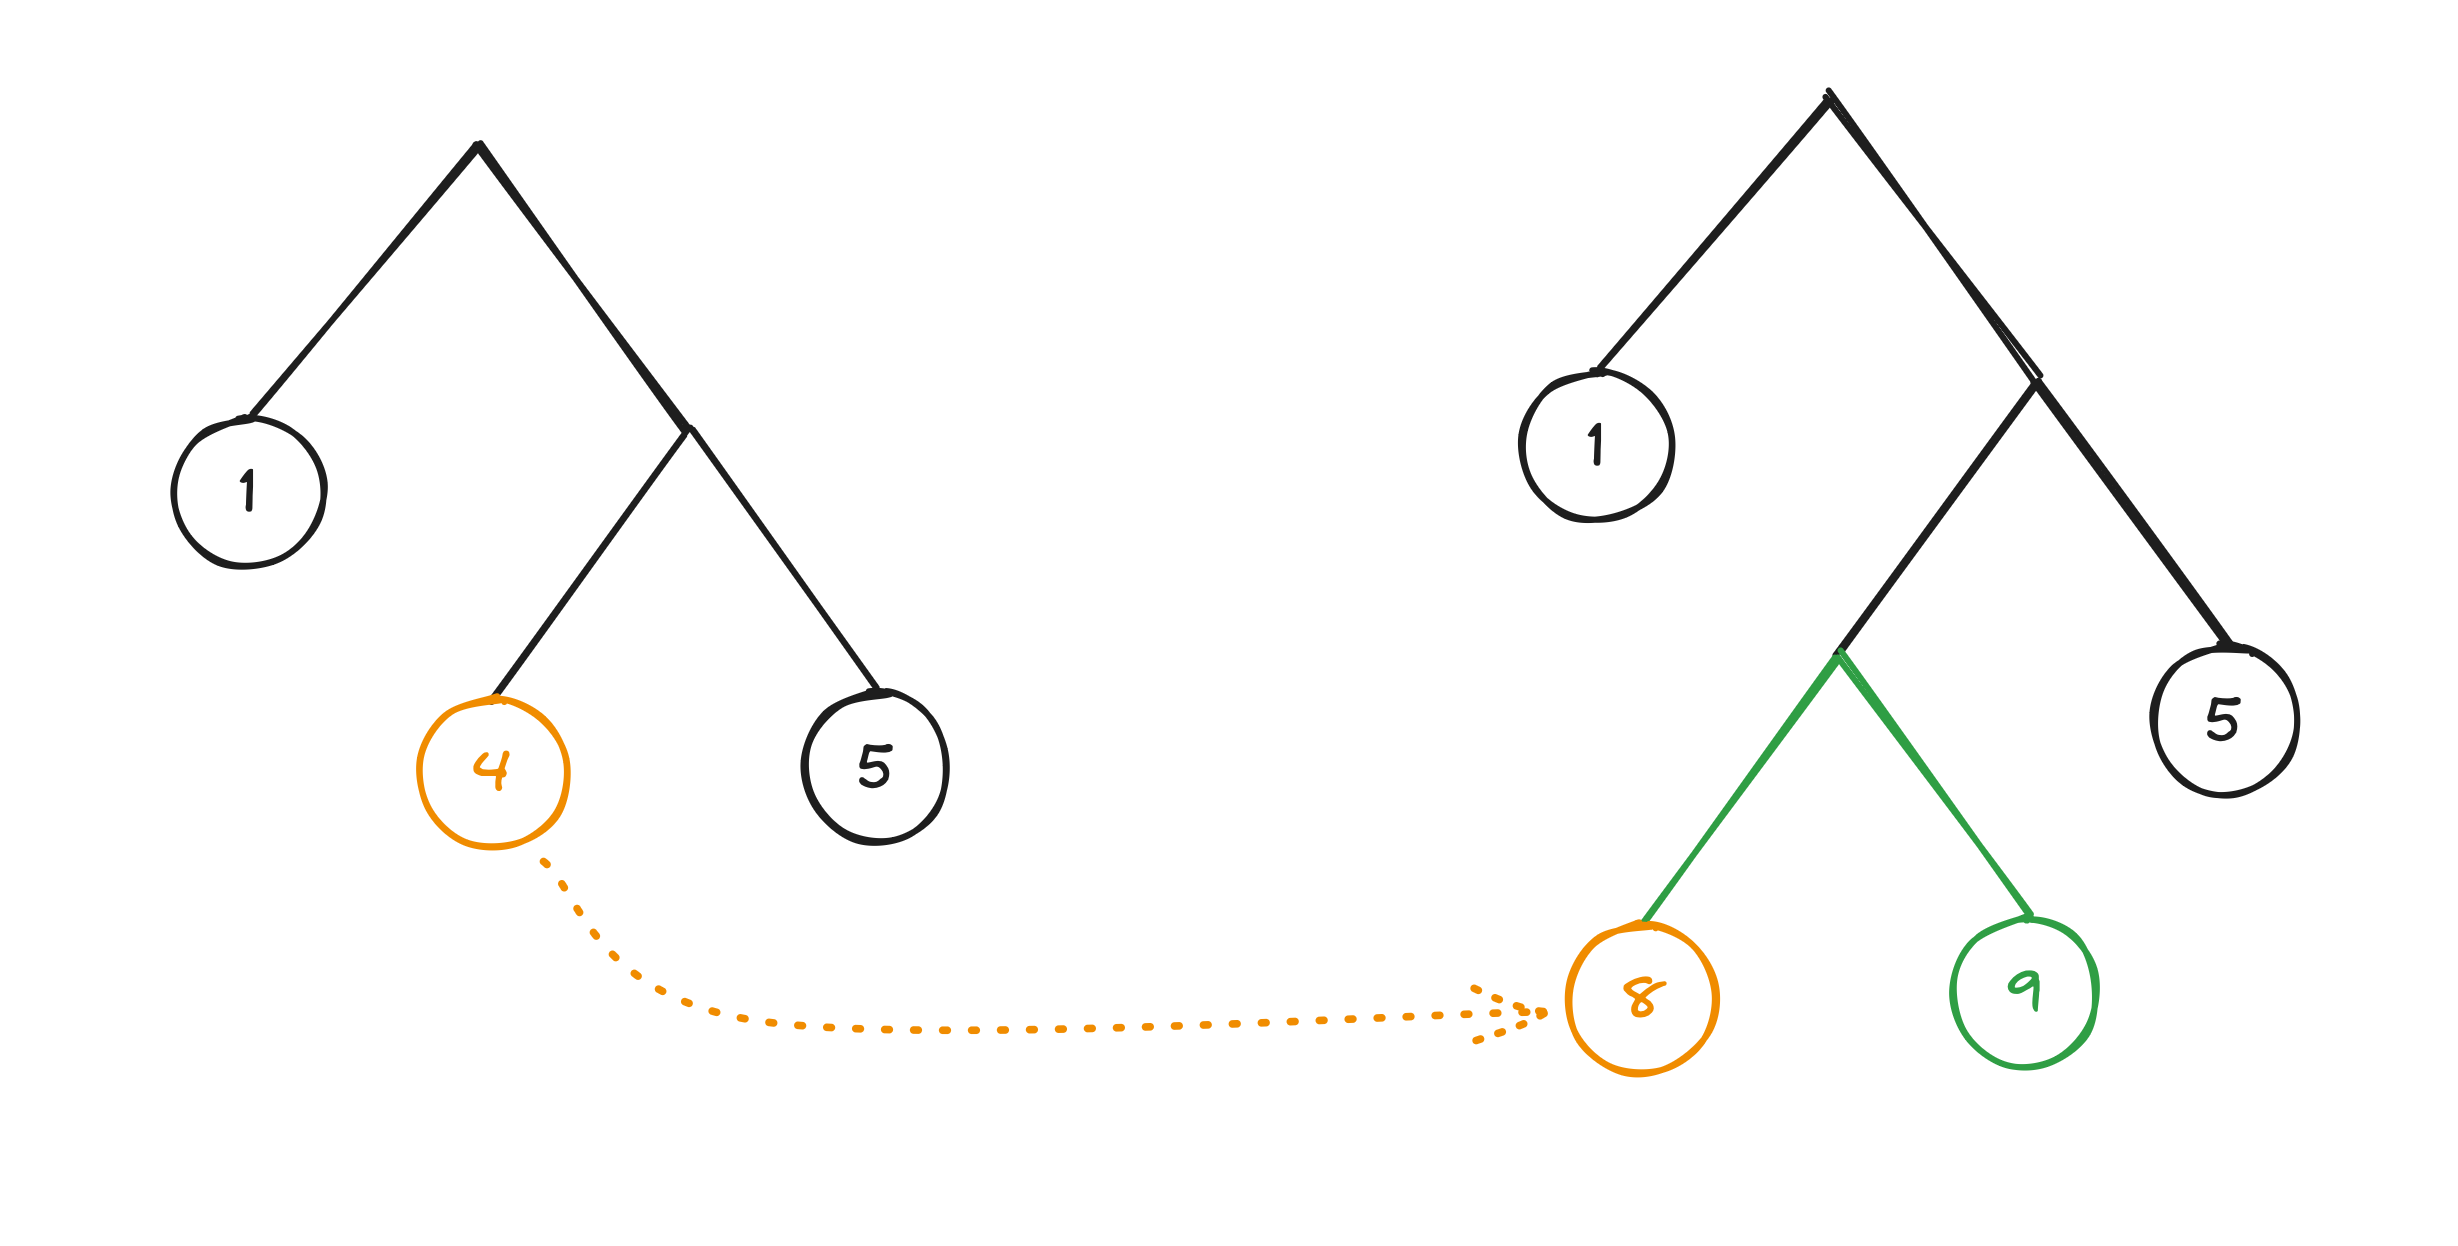
\includegraphics[width=450px, keepaspectratio]{./naive-ex.png}
  \caption{Example of an insertion with the "naive" data structure. We are inserting an element after the second priority (the one with label 4)}
  \label{naive}
\end{figure}


This solution is easy to implement and operations are fast, but it has a major drawback: the labels grow exponentially with the number of insertions and will quickly overflow.
We implemented an alternative version that uses \texttt{BigInt}s. It prevents from the overflow issue but makes the operations much slower.

\subsection{Dietz \& Sleator}

In the solution proposed by Dietz \& Sleator in 1987 \cite{10.1145/28395.28434}, we think of the set of possible labels (e.g. $0$ to $2^{64}$) as a circular list that we will fill in as we insert elements.
The priorities are connected together by a circular doubly-linked list.
The general idea for inserting a new priority after a priority \texttt{x} is the following (see Algorithm \ref{alg:dns} for more details):
\begin{itemize}
  \item We iterate through the successors of \texttt{x} and compute a weight for each of them based on the distance between the elements
  \item We stop when we reach an element whose weight is smaller than a threshold (intuitively, this means that the element is "far enough")
  \item We then relabel those elements evenly
  \item Finally, we choose a label in between the labels of \texttt{x} its successor (in the middle) and we create a new priority with this label
\end{itemize}

\begin{algorithm}
  \caption{List-range relabeling, Dietz \& Sleator} \label{alg:dns}

  \begin{algorithmic}
    \Require \texttt{x: Priority}
    \Require \texttt{base: Priority}

    \Comment{Relabel priorities}

    \State $\texttt{j} \gets 1$
    \State $\texttt{v}_0 \gets \texttt{label(x)}$
    \State $\texttt{curr} \gets \texttt{next(x)}$
    \State $\texttt{w} \gets 0$

    \While {$\texttt{w} \leq \texttt{j}^2$}
    \State $\texttt{w} \gets (\texttt{label(curr)} - \texttt{v}_0) \texttt{ \% M}$
    \State $\texttt{j} \gets \texttt{j+1}$
    \EndWhile

    \State $\texttt{to\_relabel} \gets \texttt{next(x)}$
    \For {$\texttt{k} \in 1\texttt{..}\texttt{j}$}
    \State $\texttt{label(to\_relabel)} \gets (\texttt{label(x)} + (\texttt{k} \times \texttt{w}) / \texttt{j}) \texttt{ \% M}$
    \State $\texttt{to\_relabel} \gets \texttt{next(to\_relabel)}$
    \EndFor

    \Comment{Insert the new element}

    \State $\texttt{y} \gets \texttt{new Priority}$
    \State $\texttt{label(y)} \gets ((\texttt{label(x)} - \texttt{label(base})) \texttt{ \% M} + (\texttt{label(next(x))} - \texttt{label(base)}) \texttt{ \% M})/2 $
    \State $\texttt{prec(next(x))} \gets \texttt{y}$
    \State $\texttt{next(x)} \gets \texttt{y}$

  \end{algorithmic}
\end{algorithm}

We call this algorithm \textbf{list-range relabeling}. See Figure \ref{dns} for an example.

\begin{figure}[h!]
  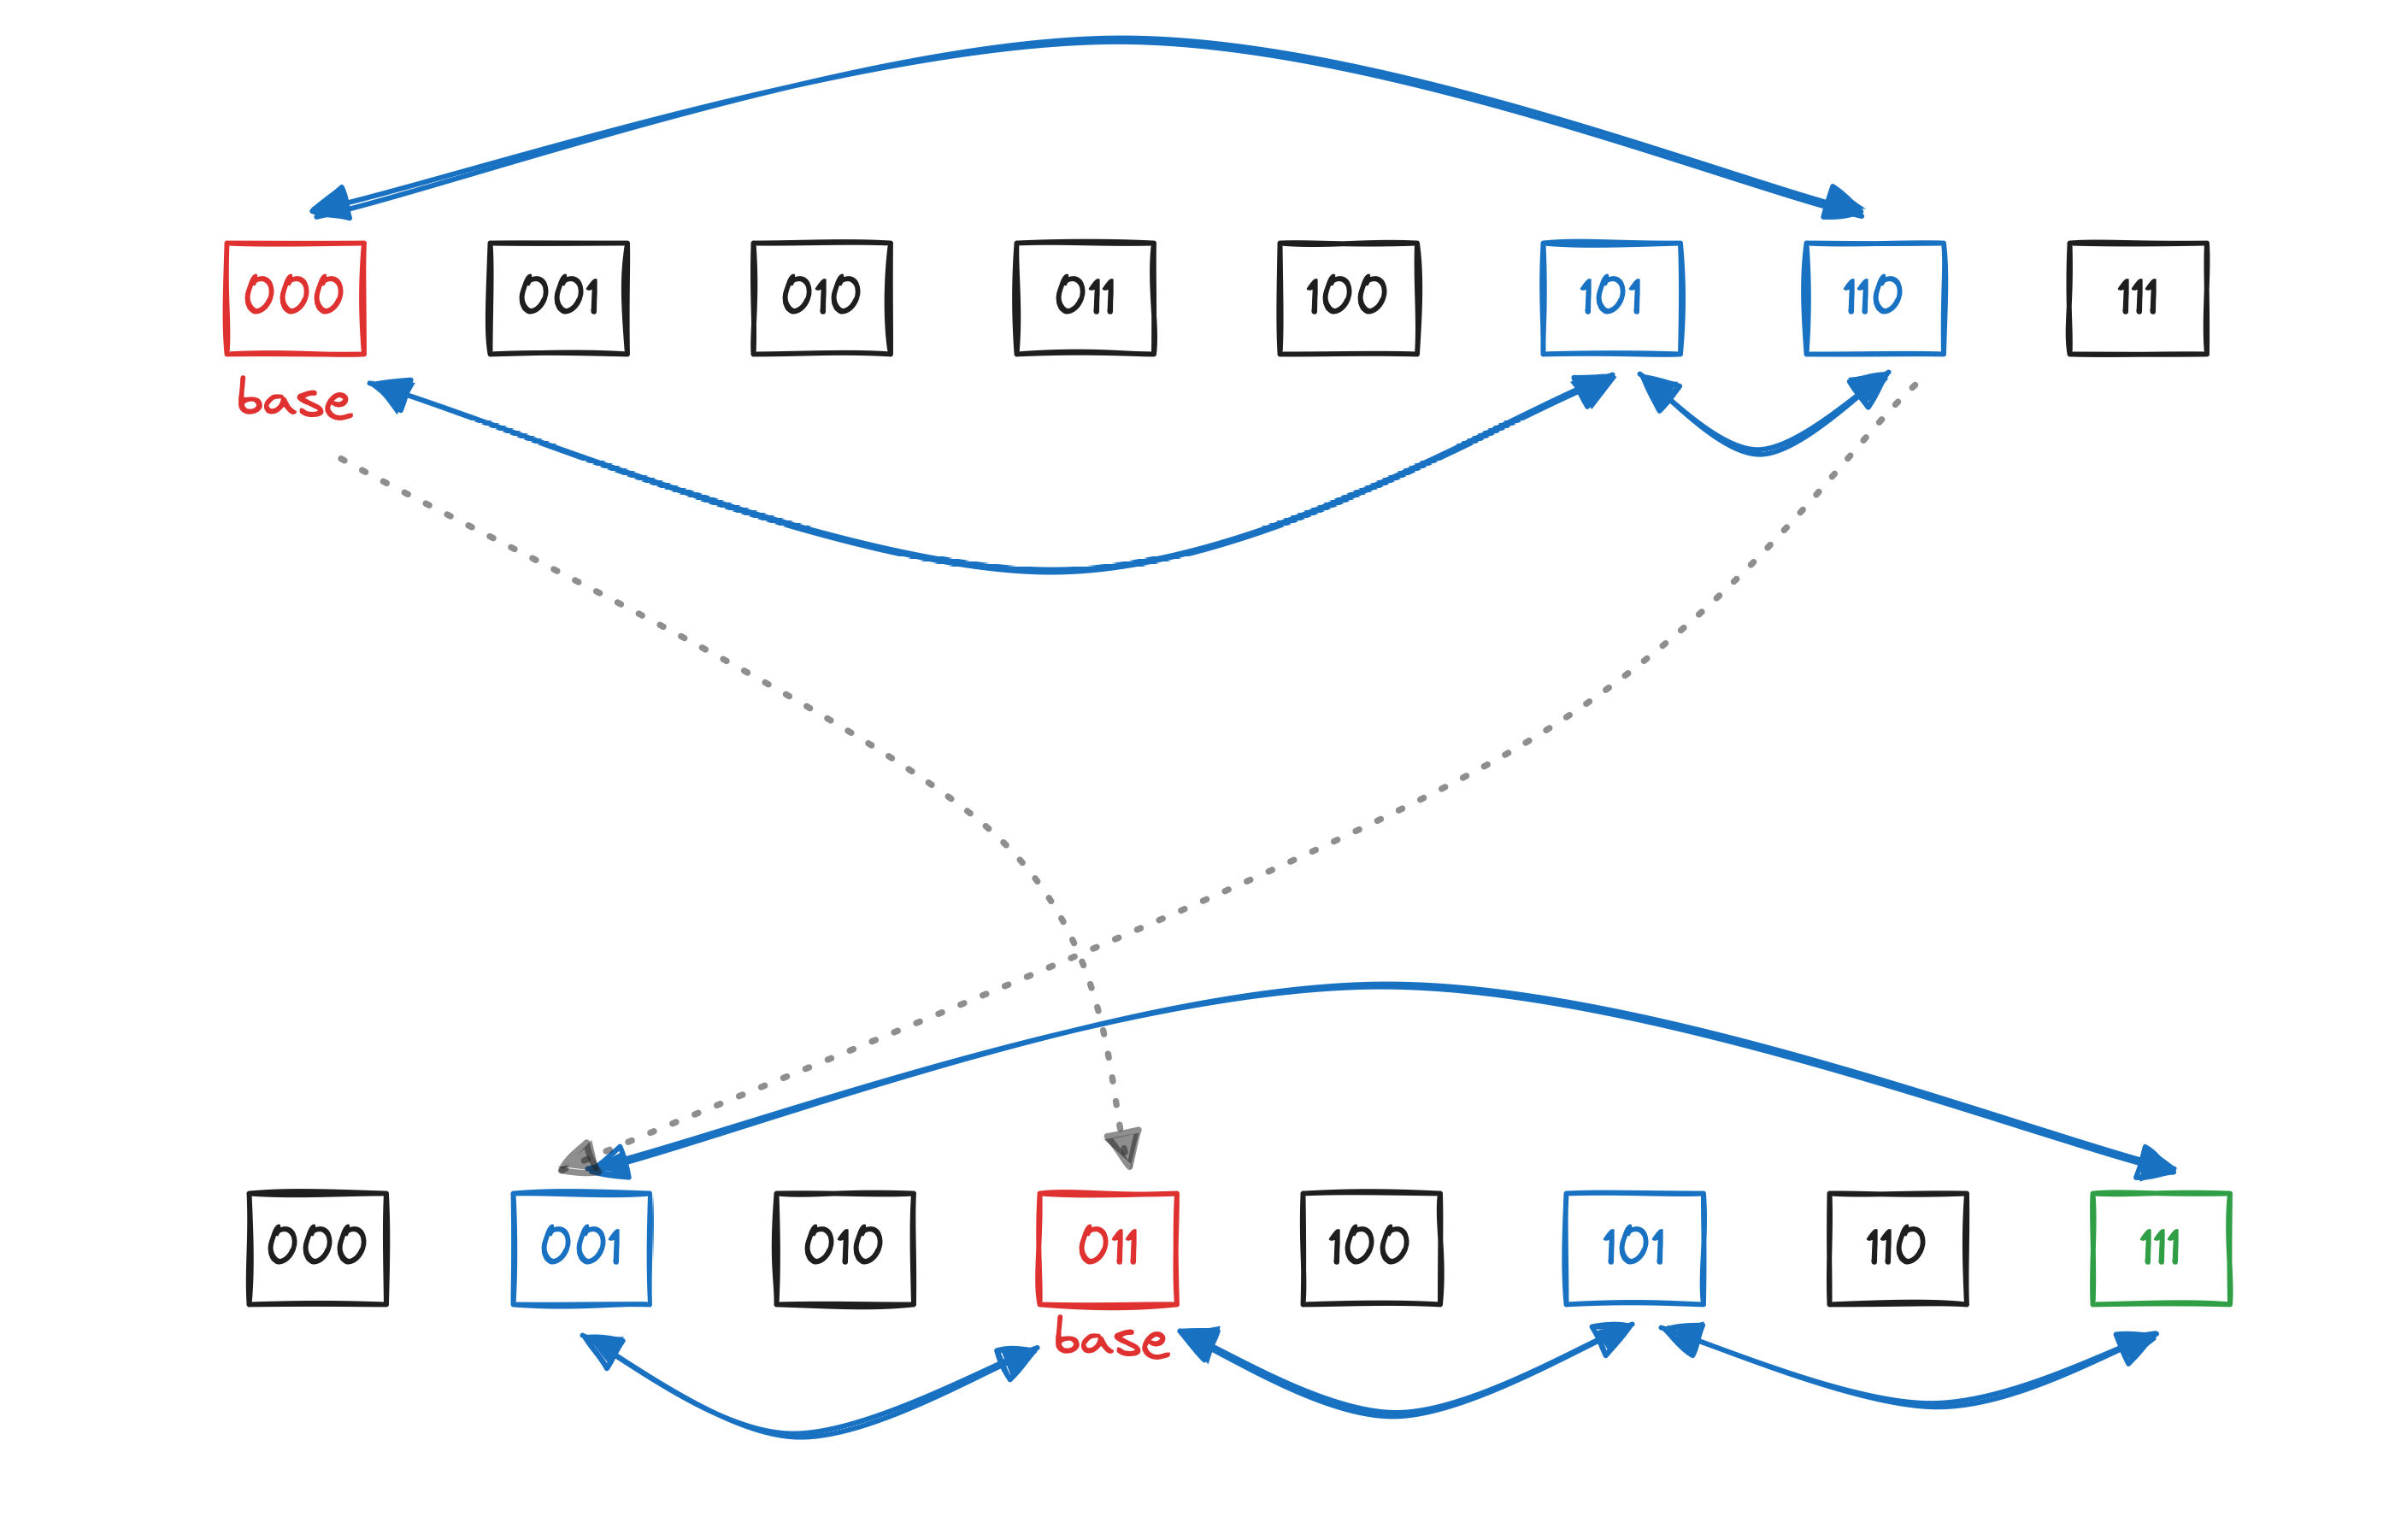
\includegraphics[width=450px, keepaspectratio]{./dns-ex.png}
  \caption{Example of an insertion with the list-range relabeling algorithm. We are inserting an element after the first element (with label 101). We can see that the base also has to move.}
  \label{dns}
\end{figure}

Note that, to avoid overflowing, we will simply loop back to 0 when we reach the maximum label ($2^{64}$).
But this means that in order to compare two elements, we have to keep track of a "base" label starting at 0 and shifting if necessary.
Then, the comparison operation is:
$$ (\texttt{label(x)} - \texttt{label(base)}) \quad \text{mod} \quad 2^{64} < (\texttt{label(y)} - \texttt{label(base)}) \quad \text{mod} \quad 2^{64} $$

Deleting an element of the data structure is as simple as removing it from the linked list.

The paper proves the following theoretical complexity bounds (where $n$ is the number of elements in the data structure):
\begin{itemize}
  \item \texttt{insert(x)}: $O(\log n)$ (amortized)
  \item \texttt{delete(x)}: $O(1)$
  \item \texttt{compare(x, y)}: $O(1)$
\end{itemize}

It is possible to get an $O(1)$ amortized complexity for \texttt{insert(x)} by adding a level of indirection using a technique by Tsakalidis \cite{10.1007/BFb0036494}. We chose not to implement this extra-layer for the sake of simplicity and because we thought that the complexity gains would be too small in comparison to the cost of the extra look-up.

This data structure theoretically only supports $\sqrt{M}$ insertions where $M$ is the number of possible labels ($2^{32}$ or $2^{64}$). It is a significant limitation on a $32$-bits machine as you can insert at most $65$K priorities.

\subsection{Bender et al.}

In 2002, Bender et al. proposed a new solution to the problem in \cite{10.5555/647912.740822}. The main goal of this approach is not to provide better bounds, but to get an algorithm and a proof that are more intuitive. In practice, we will see that our implementation is in fact faster than the first algorithm for some operations.

This time, we look at the set of possible labels ($0$ to $2^{64}$) as the leaves of a binary tree whose root is the empty string, and each node $n$ has two children $n:0 = 2 \times n$ and $n:1 = 2 \times n + 1$ (where $:$ is the concatenation to the binary representation).
We don't have to maintain an explicit tree because we can easily compute the parent or the children of a node with bit operations.
And once again, the priorities (which are leaves of the implicit tree) are connected together by a doubly-linked list (this one doesn't need to be circular).

\begin{algorithm}
  \caption{Tag-range relabeling, Bender et al.} \label{alg:bender}

  \begin{algorithmic}
    \Require \texttt{x: Priority}
    \Require \texttt{T: float (in ]1, 2[)}


    \If {$\texttt{label(x)} + 1 == \texttt{label(next(x))}$}
    \Comment{Relabeling (if needed)}

    \Comment{Find the smallest subtree that is sparse enough}

    \State $\texttt{begin} \gets \texttt{x}$
    \State $\texttt{end} \gets \texttt{x}$
    \State $\texttt{count} \gets 1$
    \State $\texttt{layer} \gets 0$
    \State $\texttt{threshold} \gets 0$
    \State $\texttt{internal\_node} \gets \texttt{label(x)}$
    \State $\texttt{min\_label\_in\_subtree} \gets \texttt{label(x)}$
    \State $\texttt{max\_label\_in\_subtree} \gets \texttt{label(x)}$


    \While{$\texttt{layer} < 64 \texttt{ \&\& } \texttt{threshold} < \texttt{count} / 2^{\texttt{layer}}$}
    \While{$\texttt{label(prec(begin))} \geq \texttt{min\_label\_in\_subtree}$}
    \State $\texttt{begin} \gets \texttt{prec(begin)}$
    \State $\texttt{count} \gets \texttt{count} + 1$
    \EndWhile
    \While{$\texttt{label(next(end))} \leq \texttt{max\_label\_in\_subtree}$}
    \State $\texttt{end} \gets \texttt{next(end)}$
    \State $\texttt{count} \gets \texttt{count} + 1$
    \EndWhile
    \State $\texttt{layer} \gets \texttt{layer} + 1$
    \State $\texttt{threshold} \gets \texttt{threshold} / \texttt{T}$

    \State $\texttt{internal\_node} \gets \texttt{internal\_node} / 2$ \Comment{Get the parent}
    \State $\texttt{min\_label\_in\_subtree} \gets \texttt{internal\_node} * 2^{\texttt{layer}}$ \Comment{Get the left-most leaf}
    \State $\texttt{max\_label\_in\_subtree} \gets \texttt{internal\_node} * 2^{\texttt{layer} + 1} - 1$ \Comment{Get the right-most leaf}
    \EndWhile

    \Comment{Relabel priorities}

    \State $\texttt{gap} \gets 2^{\texttt{layer}} / \texttt{count}$
    \State $\texttt{curr} \gets \texttt{begin}$
    \State $\texttt{curr\_label} \gets \texttt{min\_label\_in\_subtree}$

    \While {$\texttt{curr} == \texttt{next(end)}$}
    \State $\texttt{label(curr)} \gets \texttt{curr\_label}$
    \State $\texttt{curr} \gets \texttt{next(curr)}$
    \State $\texttt{curr\_label} \gets \texttt{curr\_label} + \texttt{gap}$
    \EndWhile

    \EndIf

    \Comment{Insert the new element}
    \State $\texttt{y} \gets \texttt{new Priority}$
    \State $\texttt{label(y)} \gets (\texttt{label(x)} + \texttt{label(next(x))}) / 2 $
    \State $\texttt{prec(next(x))} \gets \texttt{y}$
    \State $\texttt{next(x)} \gets \texttt{y}$




  \end{algorithmic}
\end{algorithm}

The algorithm for \texttt{insert(x)} is pretty straightforward (See Algorithm \ref{alg:bender}), and the key steps are:

\begin{itemize}
  \item if there is space ($\texttt{label(next(x))} > \texttt{label(x)} + 1$), then just insert the new element somewhere in between.
  \item if there is no space available, we have to relabel (we call this algorithm \textbf{tag-range relabeling}).
        \begin{itemize}
          \item To do so, we simply have to go up the tree and find the first sub-tree containing \texttt{x} that is not "too dense".
          \item Once we find this sub-tree, we evenly spread all the elements it contains over the range of labels of the sub-tree. Note that once again, all these operations can be done with simple bit manipulations over the labels.
        \end{itemize}
\end{itemize}

See Figure \ref{bender} for an example.

\begin{figure}[h!]
  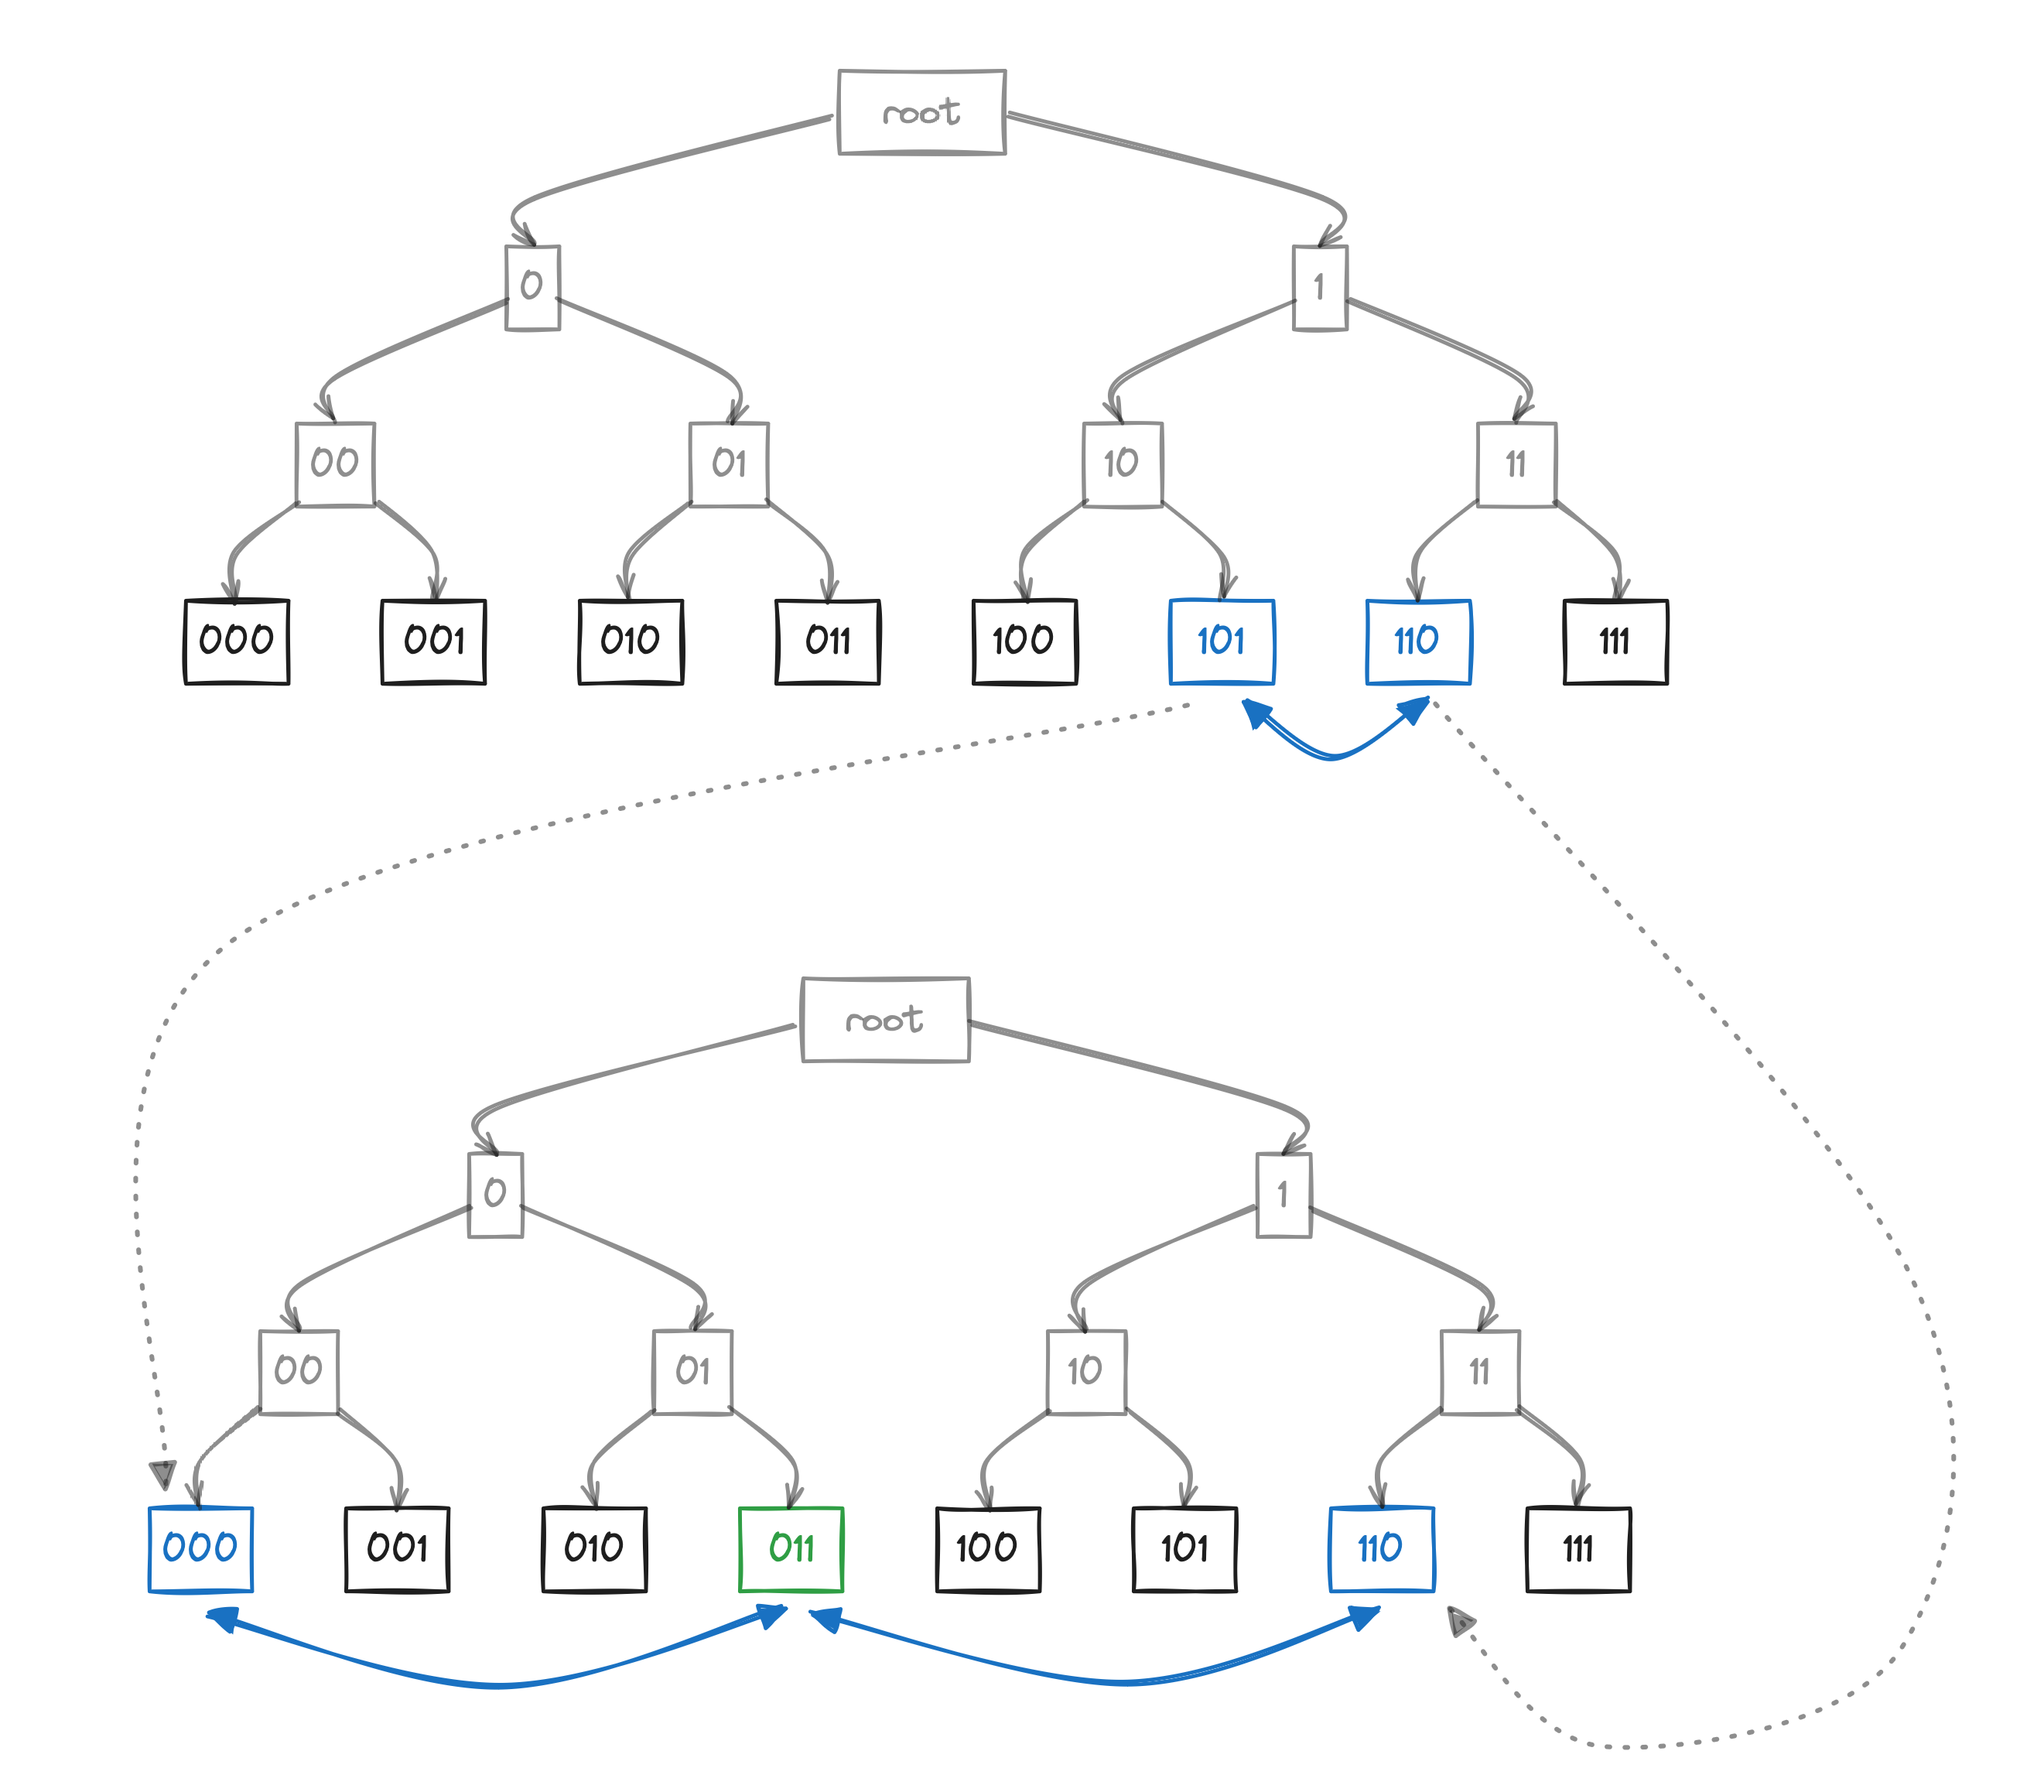
\includegraphics[width=450px, keepaspectratio]{./bender-ex.png}
  \caption{Example of an insertion with the tag-range relabeling algorithm. We are inserting an element after the first element (with label 101). The first sub-tree that was sparse enough is the whole tree (assuming we chose \texttt{T} accordingly).}
  \label{bender}
\end{figure}

The paper proves that this algorithm has the same complexity bounds as the previous one:
\begin{itemize}
  \item \texttt{insert(x)}: $O(\log n)$
  \item \texttt{delete(x)}: $O(1)$
  \item \texttt{compare(x, y)}: $O(1)$
\end{itemize}

The same indirection trick can be applied to reduce the insertion's complexity, but we chose not to implement it for the same reasons as before.

Deleting an element of the data structure is as simple as removing it from the linked list.
And a small but important difference is that, in order to compare two elements, we simply have to compare their labels (and we don't have to compute their position relative to a base as in the previous solution).

The previous data structure was limited to $\sqrt{M}$ insertions. Here, the maximum number of elements you can insert depends on the parameter $T$. If $T$ is close to $2$, the insertion will be faster but you can only insert a small amount of priorities before the root overflows. If $T$ is close to $1$, the algorithm is slower but you can insert more priorities (close to $M$).
The issue is that it's difficult to find a good trade-off as the user doesn't usually know up-front how many priorities he will need.
But the good news is that $T$ doesn't have to be fixed and you can compute the best $T$ at each insertion.
This computation is not free though, and we will see later (section \ref{precompute}) how we made this process faster.

\newpage
\section{Implementation}

In this section, I will present the main data structures and design choices of our implementations, as well as some tricks we used to improve the speed.

\subsection{Interface}

The project was built as a Rust library (a \lstinline{cargo crate}). In order to have a common interface for multiple implementations, as well as shared tests and benchmarks, we leveraged Rust's \lstinline{Trait} system. The interface for a priority is minimal:
\begin{itemize}
  \item \lstinline{new: () -> Priority}: create a new priority, unrelated to any other priority
  \item \lstinline{insert: Priority -> Priority}: insert a new priority right after the argument
\end{itemize}

The comparison is made possible through the implementation of the \lstinline{PartialCmp} trait which lets us use the common comparison operators (\lstinline{>=}, \lstinline{<}, etc.).

The deletion is implemented through the \lstinline{Drop} trait, which acts as a destructor. A priority is deleted from the data structure when it goes out of scope.

\subsection{Common data structures}

I won't go too much into the technical details, but we used a couple of data structures to implement both solutions (\cite{10.5555/647912.740822} and \cite{10.1145/28395.28434}).

\begin{itemize}
  \item \lstinline{PriorityInner} is a node of a circular doubly-linked list. It can be seen as the private interface of a \lstinline{Priority}. It stores the following fields: \lstinline{prev}, \lstinline{next}, \lstinline{label}, \lstinline{ref_count}. The first two are (smart) pointers to the neighbors, the third is the label as a \lstinline{usize = u64} (on a 64-bit machine), and the last one is used for the manual reference counting. Those fields are actually wrapped in smart pointers called \lstinline{RefCell}, mutable memory locations. It is necessary to abide by Rust's borrow checker when trying to mutate a field of an object that is not owned or borrowed as mutable (this is called the interior mutability pattern).
  \item \lstinline{Arena} is the internal store of priorities containing all the \lstinline{PriorityInner}. In our case, it's a \lstinline{Slab}. It is indexed by \lstinline{PriorityKey}, an alias for \lstinline{usize}. The implementation of the \lstinline{Arena} contains all the methods in charge of creating, deleting, and connecting the \lstinline{PriorityInner}, the nodes of the linked list.
\end{itemize}

The end-user has access to a \lstinline{Priority}, which contains (privately) its \lstinline{PriorityKey} and a reference to the \lstinline{Arena}.

\subsection{Pre-computing the density thresholds} \label{precompute}

When looking at Algorithm \ref{alg:bender}, you might notice some potentially expensive operations.
First, we have many multiplications and divisions by powers of $2$ used to traverse the tree. Those are not an issue since we can simply use the efficient right- and left-shifts operations (\texttt{>>}, \texttt{<<}).

The more annoying ones are the floating point operations needed to compute the density threshold.
\texttt{T} is a parameter between $1$ and $2$ and the maximum density of a subtree whose root has a height $h$ ($0$ being the height of a leaf) is $\texttt{T}^{-h} = 1 / \texttt{T}^h$.
It gets even worse if we compute the best value for $T$ at each insertion to ensure the algorithm terminates without compromising its speed.

The solution we chose was to pre-compute some values at compile time that the algorithm will simply have to look-up.
The values that we need are
$$[\texttt{T}^{-i} \texttt{  for i in 0..64  for T in list\_of\_Ts}]$$
where \texttt{list\_of\_Ts} is a list of numbers between $1$ and $2$. In our case we chose $20$ values evenly distributed between $1.1$ and $1.9$.
However, there are still two issues remaining: We still have to compute the densities of the subtrees (float) at run-time, and we don't have an easy way of finding which value of \texttt{T} we should use.

To solve these, instead of pre-computing the density thresholds, we chose to calculate the (integer) capacities of the subtree for different heights $h$ and values of \texttt{T}:
$$ \left\lfloor \frac{2^h}{T^h} \right\rfloor $$
This value can simply be compared to the number of priorities contained in the subtree.
Moreover, it's now trivial to find the best \texttt{T} by finding the capacity that is closest to (and larger than) the total number of priorities in the \texttt{Arena}.


\newpage
\section{Testing, Benchmarking, and results}

\subsection{Unit tests, Integration tests, and Quickcheck}

We implemented a pretty large test suite in order to ensure the correctness of the implementations. It was a good idea given the number of bugs we were able to find thanks to these tests.

\begin{itemize}
  \item Unit tests: We implemented to test the various internal data structures, and in particular make sure we were not leaking any memory in the process.
  \item Integration tests: We implemented multiple scenarii using the public methods of a \texttt{Priority}. The interface is really simple (insertion, deletion, comparison), making the testing process straightforward.
  \item Quickcheck: The simplicity of the interface encouraged us to try a random and automated property-based testing tool called Quickcheck (it's the Rust port of a Haskell library). The general idea is that we simply have to implement the \texttt{Arbitrary} trait for our data structure and define some properties that must be true for any instance of the data structure.

        Our first approach was to generate an arbitrary \texttt{Vec<Priority>} by inserting and deleting priorities and maintaining the order of the vector. The only property we have to check is: "Is the order of the vector the same as the order of our data structure?".
        One nice feature of Quickcheck is the shrinking, meaning that it will try to find a minimal example by shrinking the failing input.
        But we can't "reverse" an insertion or a deletion, the internal state will be different.

        The solution is to generate arbitrary vectors of decisions that can be either \texttt{Insert(i)} or \texttt{Delete(i)} for an index \texttt{i}. We turn this vector of decisions into a vector of priorities only when the property is tested.
        Shrinking the vector of decision can be done by removing the decisions from the end until we find the one that caused the failure.
\end{itemize}

\subsection{Bugs found and fixed}

We found multiple bugs thanks to our tests. Most of them were found by Quickcheck, giving confirmation that human programmers are pretty bad at testing edge cases.
In particular we fixed two bugs related to integer overflow. In both implementations, we used word-sized labels to optimize memory and speed. When manipulating the labels, we thus had to be careful not make mistakes (in particular in \cite{10.1145/28395.28434} which uses modular arithmetic).

The first "interesting" bug was found in the implementation of \cite{10.5555/647912.740822}, when trying to compute the minimum and maximum label of a subtree. Given an internal node with label $x$ at height $i$, the minimum is $x \cdot 2^i = x >> i$ and the maximum is $x \cdot 2^{i+1} - 1 = (x + 1) >> i$. This calculation overflows if the subtree is the right-most one. Our solution was to notice that the maximum was simply the label of internal node with $i$ "$1$" at the end. This can be written $!((!x) >> i) $.

The second bug happened in the implementation of \cite{10.1145/28395.28434}. When relabeling the nodes, the paper simply suggests to compute the value
$$\left\lfloor \frac{k \cdot w}{j} \right\rfloor \% M$$
The problem is that  $k\cdot w$ might overflow. Initially, we were computing
$$\left\lfloor \frac{(k \cdot w) \% M}{j} \right\rfloor$$
At first, we didn't realize that they were different. It turns out that division in modular arithmetic is a bit trickier than we thought
$$(a/b)\%M = (a\%M \cdot b^{-1}\%M)\%M $$
where $b^{-1}$ is the modular inverse of $b$ (such that $(b \cdot b^{-1}) \%M = 1$).
$b^{-1}$ can be computed with the extended Euclidean algorithm in $O(\log^2(M))$. In practice and for the sake of simplicity, we instead chose to locally cast the numbers to 2-words integers and perform the overflowing calculation, before casting it back to \texttt{usize}. Our benchmarks indicated it didn't have any measurable impact on speed.

\subsection{Benchmarks, Profiling, and Optimization}

Our benchmarks were mainly aimed at comparing the implementations on two tasks: insertion and comparison. We used the crate \texttt{Criterion} to write and execute the benchmarks (including precise measurements).

Benchmarking the insertion gave us multiple insights:


\begin{table}[h!]
  \begin{center}
    \begin{tabular}{|c | c c c c|}
      \hline
      \#insertions & list-range & tag-range & naive & naive-bigint \\ [0.5ex]
      \hline
      10           & 60         & 63        & 75    & 150          \\
      \hline
      1\_000       & 31         & 37        &       & 122          \\
      \hline
      100\_000     & 47         & 46        &       & 140          \\
      \hline
      1\_000\_000  & 156        & 155       &       &              \\
      \hline
      5\_000\_000  & 188        & 185       &       &              \\
      \hline
    \end{tabular}

    \caption{Time per insertion (nanoseconds) depending on the total number of insertions}
    \label{table:insert}

  \end{center}
\end{table}

When inserting at random, our implementations of \cite{10.1145/28395.28434} and \cite{10.5555/647912.740822} have the same performance (see Table \ref{table:insert}). This is in line with the results presented in \cite{10.5555/647912.740822}. However, the list-range relabeling is a bit faster for some common edge cases such as "always insert after the last element".

It is also important to mention that the list-range relabeling has a strict limit in terms of how many priorities you can insert whereas the tag-range relabeling (with the variable threshold discussed above) can use almost every possible label for a given word size.

We were also able to measure the average insertion time for different total number of insertions (see Figure \ref{graph:insert}). \cite{10.5555/647912.740822} showed that the average number of relabeling was increasing with the total number of elements inserted, and this is in line with the speed we measured.

\begin{figure}[h!]
  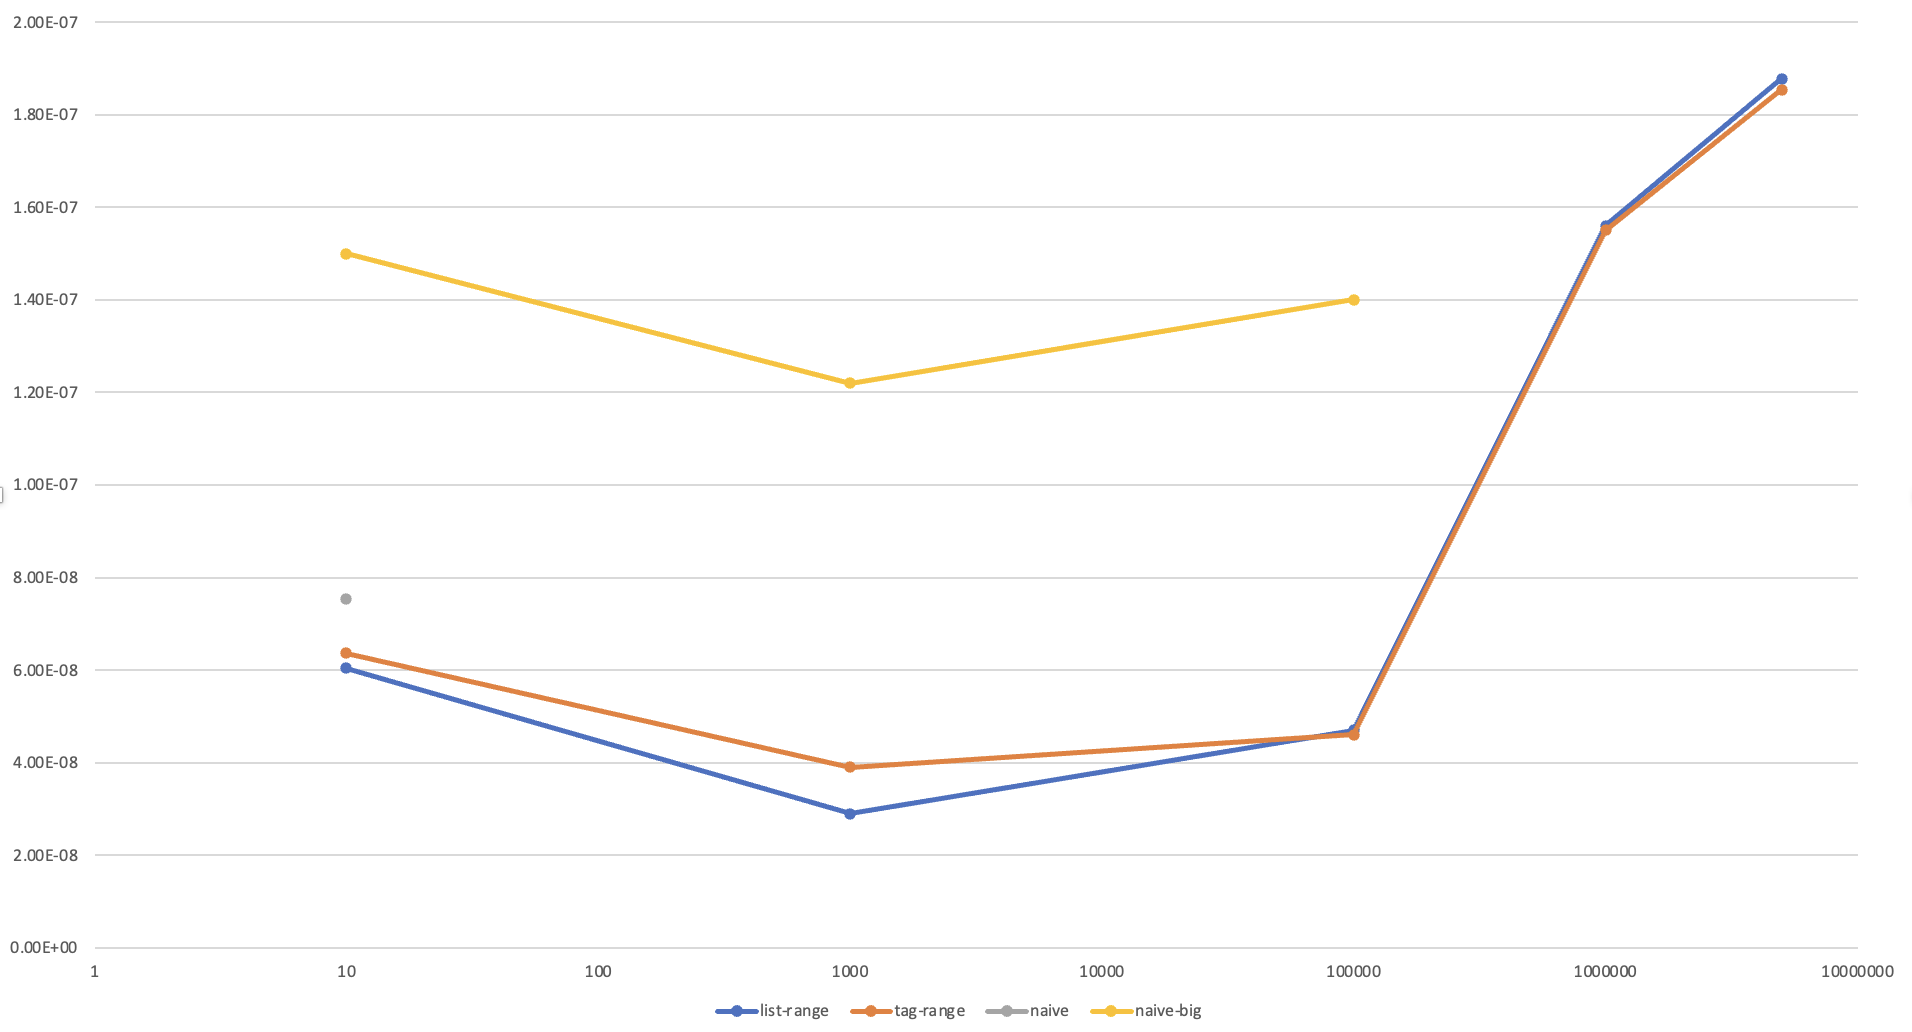
\includegraphics[width=450px, keepaspectratio]{./insert.png}
  \caption{Time per insertion (nanoseconds) depending on the total number of insertions}
  \label{graph:insert}
\end{figure}

The naive algorithm using word-sized labels has approximately the same speed as our other implementations but it is limited to a very small total number of insertions. We also tried to extend this naive approach using \texttt{BigInt}s. As visible on the graph, this is a lot slower.

We also created two benchmarks to measure the comparison speed. One that creates priorities (with insertions and deletions to "shuffle" the slab and avoid too much gains due to caching) and then compares two random priorities, and another one that also creates a random vector of $200$ priorities but this time sorts it (see Table \ref{table:comparison}).

\begin{table}[h!]
  \begin{center}
    \begin{tabular}{|c | c c c c|}
      \hline
      benchmark & list-range & tag-range & naive & naive-bigint \\ [0.5ex]
      \hline
      compare2  & 8.3        & 5.2       & 11    & 200          \\
      \hline
      sort      & 3221       & 2645      &       & 43672        \\
      \hline
    \end{tabular}

    \caption{Time per comparison or sort (nanoseconds)}
    \label{table:comparison}

  \end{center}
\end{table}

We notice that the naive implementation is slower than the others, which is great since that means we are not making adding unnecessary if the user only needs a small amount of priorities.

Another important take-away is that the tag-range algorithm (\cite{10.5555/647912.740822}) is faster than the other in terms of comparison speed. This makes sense: the comparison in the tag-range version is 2 look-ups and 1 comparison whereas in the list-range version, you need 3 look-ups (you need the label of the base), 2 wrapping substraction, and 1 comparison.

In order to find bottlenecks in our code, we performed some profiling using the \texttt{cargo-flamegraph} crate. This library is really easy to use, can be plugged to benchmarks, and produces useful graphs at a "function granularity" (e.g. Figure \ref{graph:flame}). We sometimes had to artificially refactor our code into very small functions to get a more detailed output.

\begin{figure}[h!]
  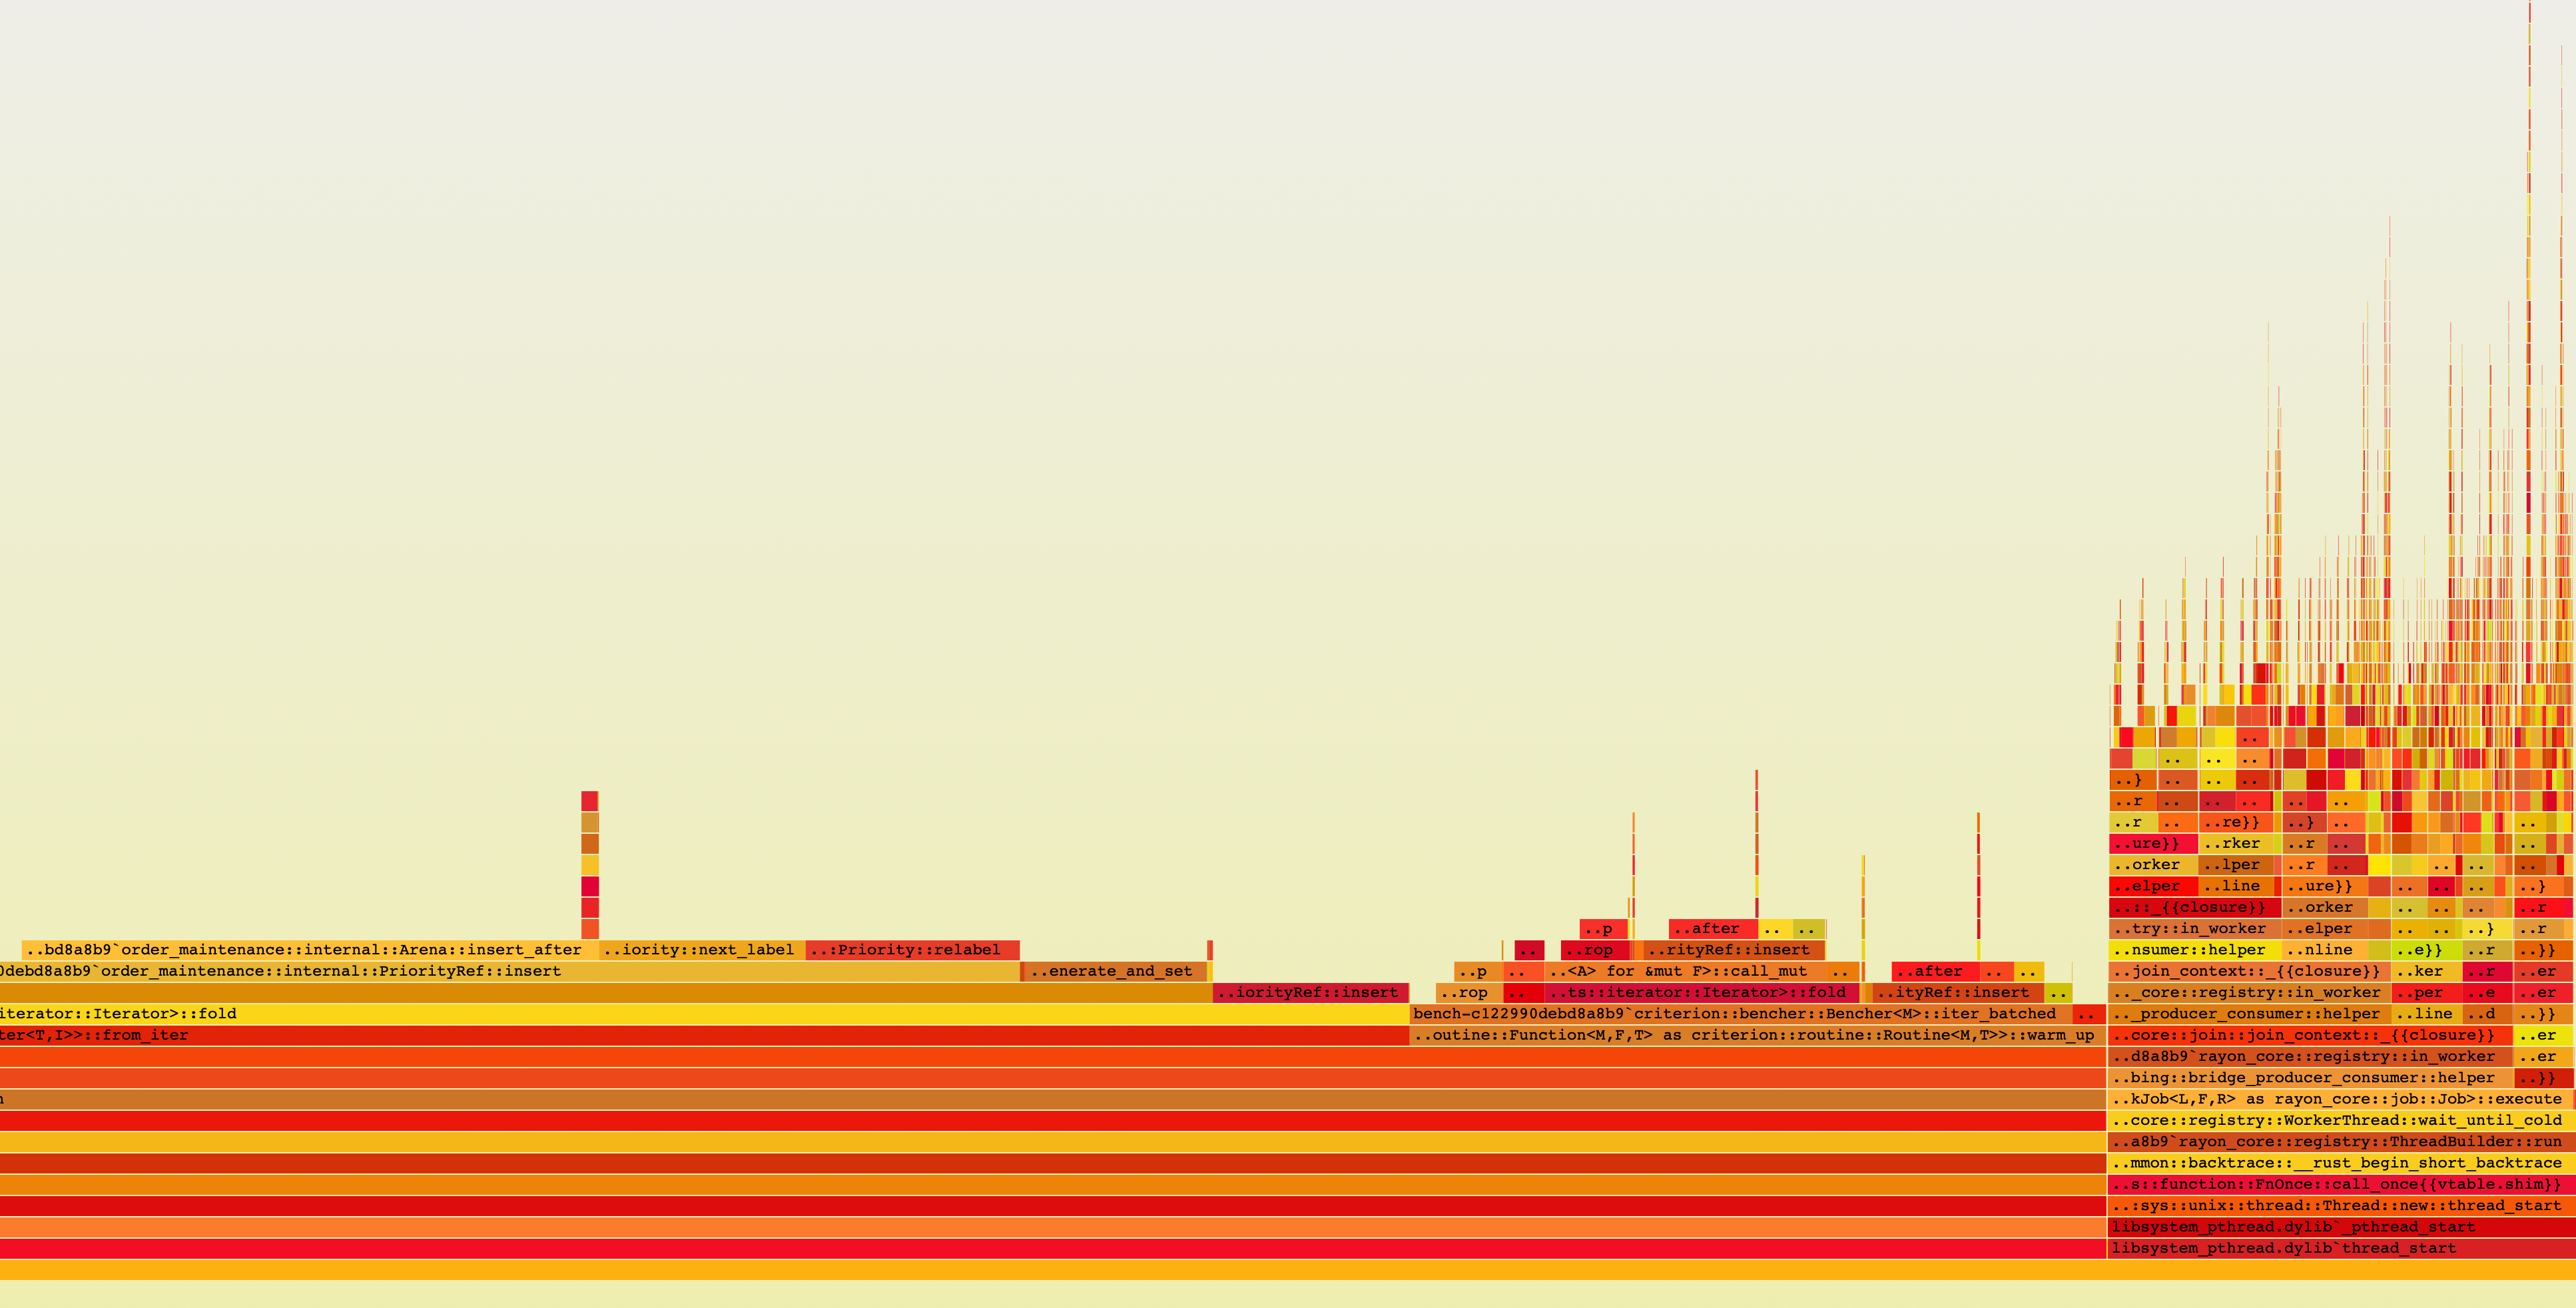
\includegraphics[width=450px, keepaspectratio]{./flamegraph.png}
  \caption{Example of a flamegraph produced by the crate}
  \label{graph:flame}
\end{figure}

Thanks to these flamegraphs, we were able to optimize some parts of the implementations. For example:
\begin{itemize}
  \item Using a \texttt{Slab} to store the priorities was approximately 20\% faster (on our benchmarks) than using a \texttt{SlotMap} that we initially used.
  \item To compute the mid-point between two labels, it's 15\% faster (on my laptop) to use integers operations (\texttt{x + (y-x)/2}) rather than using bit manipulation (\texttt{(x\textasciicircum y) >> 1 + x\&y}). This one was unexpected, we thought the two would be equivalent after the compiler optimizations.
\end{itemize}

\newpage
\section{Conclusion and Future Work}

This project led to the development of an (almost) production-ready Rust library. We were able to verify or refine the theoretical claims of the papers on real-world use-cases.

The current conclusion is that we should use the implementation of the algorithm from \cite{10.5555/647912.740822}, as it is simple to understand and maintain, and provides better or similar results on every benchmark.

There are still some areas to explore in the future. Among them:
\begin{itemize}
  \item Testing and benchmarking on a microcontroller, since it was one of the initial motivations of this project. Our hope is that we will see similar trends on different hardware.
  \item Trying out different allocation strategies. We already experimented with multiple stores, but this analysis could be refined. It might also be worth trying using \texttt{UnsafeCell} instead of \texttt{RefCell} now that we are more confident about the correctness of the code.
  \item Adding a level of indirection. Both papers reduce the theoretical complexity by adding a level of indirection. Our guess is that it wouldn't improve the speed because of the cost of the additional look-ups, but it might be worth trying.
\end{itemize}

I also wanted to address special thanks to John who has been extremely patient and helpful this semester!

\newpage
\printbibliography

\end{document}

